\section{Étude de la dynamique du Pendule Inversé}

\begin{frame}
\frametitle{Étude de la dynamique}
\framesubtitle{Présentation du système}

\begin{figure}
    \only<1>{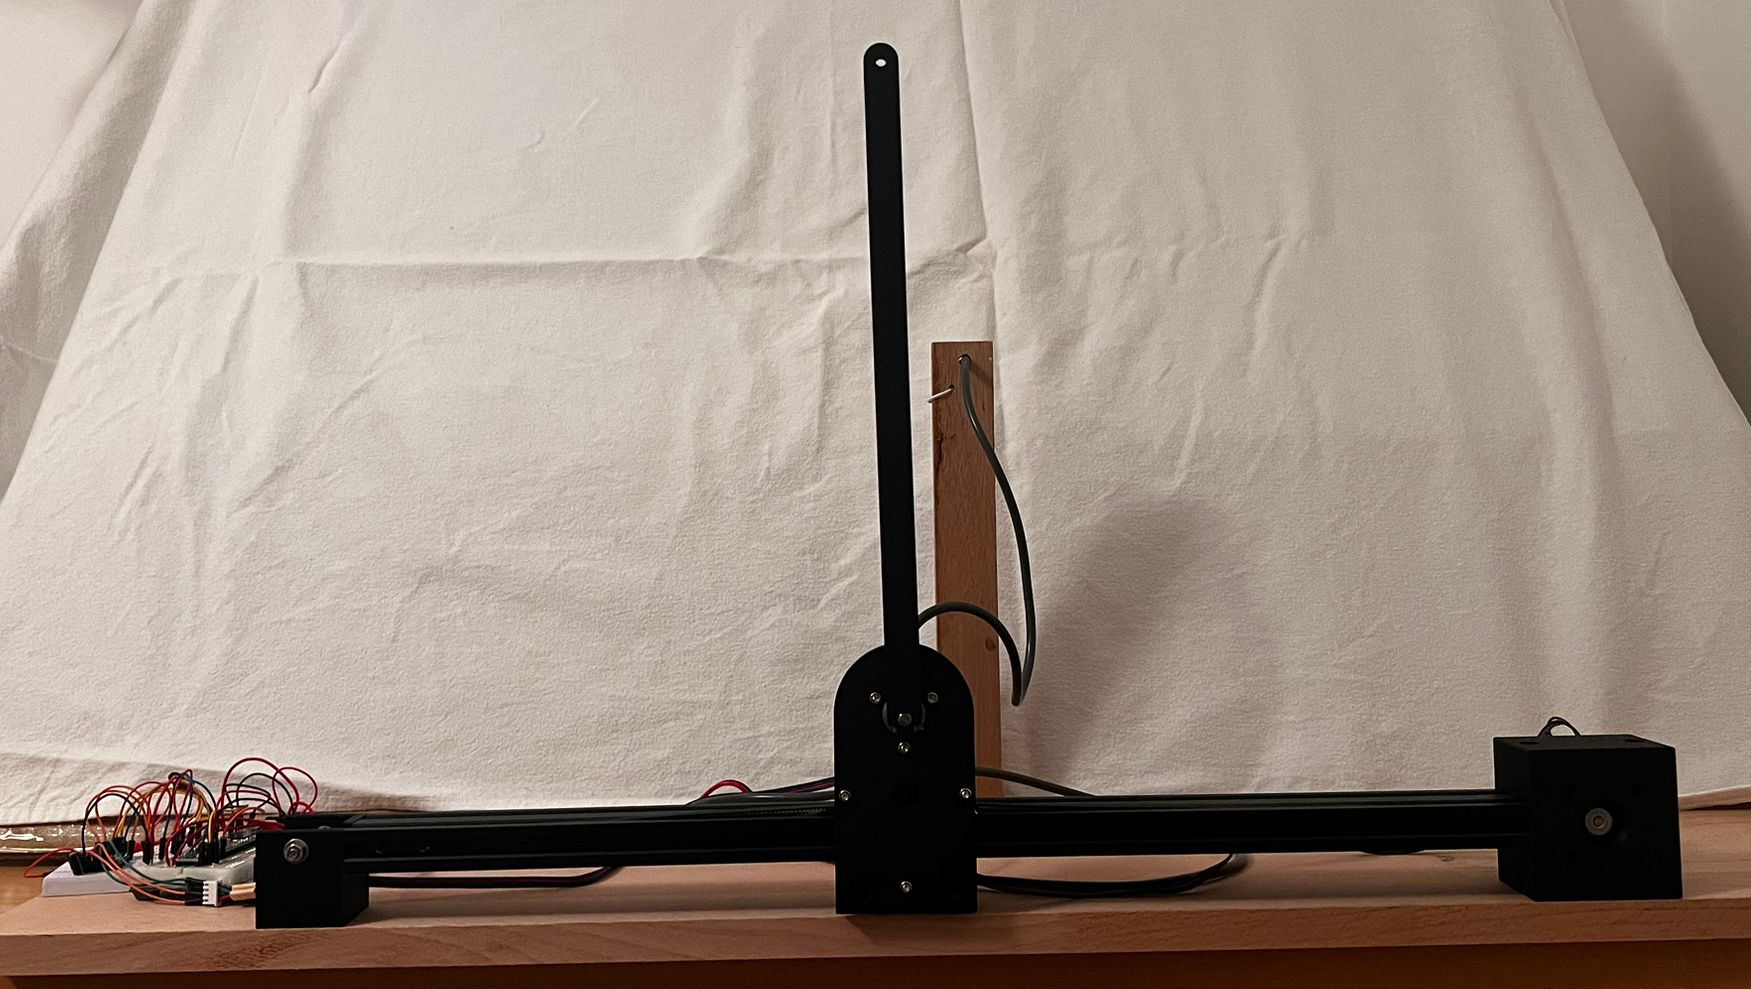
\includegraphics[width=\textwidth]{figures/pendulum-picture.jpg}}%
    \only<2>{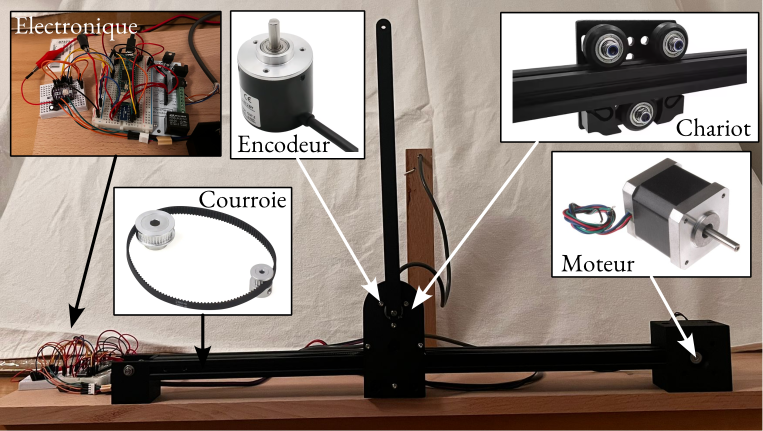
\includegraphics[width=\textwidth]{figures/inverted_pendulum_picture_schematic.png}}
\end{figure}

\end{frame}

%%%%%%%%%%%%%%%%%%%%%%%%%%%%%%%%%%%%%%%%%%%%%%%%

\begin{frame}
\frametitle{Étude de la dynamique}
\framesubtitle{Modèle et Équations de la dynamique}

\begin{columns}[T]

%--- Colonne gauche : schéma ---
\begin{column}{0.45\textwidth}
\begin{center}
\begin{tikzpicture}[>=Stealth, scale=0.8]

  % Ground
  \fill[pattern=north east lines, pattern color=gray!60] (-1.5,-0.18) rectangle (1.5,0);
  \draw[thick] (-1.5,0) -- (1.5,0);

  % Wheels
  \draw[thick, fill=white] (-0.45, 0.15) circle [radius=0.15];
  \draw[thick, fill=white] ( 0.45, 0.15) circle [radius=0.15];

  % Cart body
  \draw[thick, fill=gray!20, rounded corners=3pt]
    (-0.8, 0.15) rectangle (0.8, 0.75);

  % Pivot
  \coordinate (O) at (0, 0.75);
  \fill (O) circle [radius=0.1];

  % Pendulum (theta = 150 deg from downward, 30 deg from upright)
  \coordinate (tip) at ($(O) + ({0.5*3.0}, {0.866*3.0})$);

  % Dashed verticals
  \draw[dashed, gray] (O) -- ++(0,  3.5);
  \draw[dashed, gray] (O) -- ++(0, -0.9);

  % Angle arc (CCW from downward to rod, through right side)
    \draw[->] ($(O)+(-90:0.7)$) arc[start angle=-90, end angle=60, radius=0.7] node[near end, right] {$\theta$};

  % Pendulum rod
  \draw[line width=2pt] (O) -- node[midway, right=6pt] {$m,I$} (tip);

  % Length arrow
  \draw[<->, thin]
    ($(O)   + ({-0.866*0.35}, {0.5*0.35})$)
    -- node[left=2pt] {$l$}
    ($(tip) + ({-0.866*0.35}, {0.5*0.35})$);

  % Tip dot
  \fill (tip) circle [radius=0.05];

  % Acceleration arrow
  \draw[->, very thick, blue!70!black]
    (0.85, 0.44) -- ++(1.0, 0) node[right] {$u = \ddot{x}$};

\end{tikzpicture}
\end{center}
\end{column}

%--- Colonne droite : équations ---
\begin{column}{0.52\textwidth}
  \vspace{0.5cm}
  \textbf{Équation du mouvement :}
  \begin{equation*}
    D\,\ddot{\theta} + c\,\dot{\theta} + mgl\sin\theta + ml\cos\theta\cdot u = 0
  \end{equation*}
  avec $D = I + ml^2 = \dfrac{4}{3}ml^2$
\end{column}

\end{columns}

\end{frame}

%%%%%%%%%%%%%%%%%%%%%%%%%%%%%%%%%%%%%%%%%%%%%%%%

\begin{frame}
\frametitle{Étude de la dynamique}
\framesubtitle{Linéarisations et Réponses du système}

\begin{columns}[T]

\begin{column}{0.48\textwidth}
  \centering\textbf{Position basse} ($\theta \approx 0$)
  \begin{equation*}
    D\,\ddot{\theta} + c\,\dot{\theta} + mgl\,\theta = 0
  \end{equation*}
  $\Rightarrow$ Oscillations amorties

  \begin{figure}
      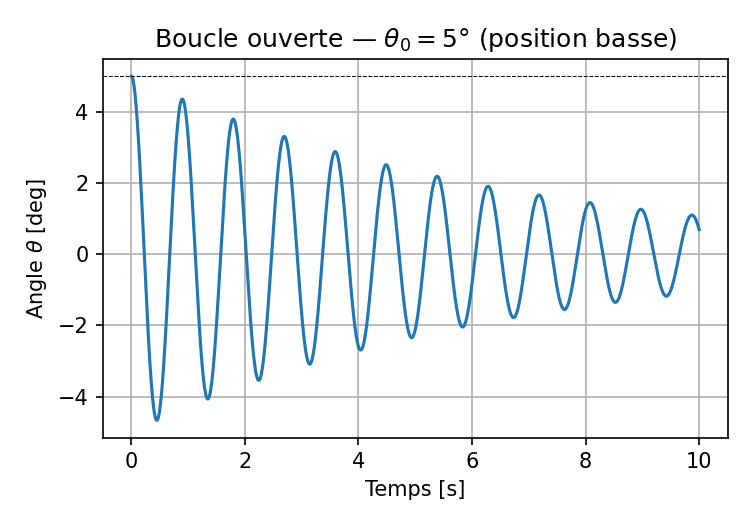
\includegraphics[width=\linewidth]{figures/openloop_5deg.png}
  \end{figure}
\end{column}

\begin{column}{0.48\textwidth}
  \centering\textbf{Position haute} ($\varphi = \theta - \pi \approx 0$)
  \begin{equation*}
    D\,\ddot{\varphi} + c\,\dot{\varphi} - mgl\,\varphi = 0
  \end{equation*}
  $\Rightarrow$ Divergence exponentielle

  \begin{figure}
      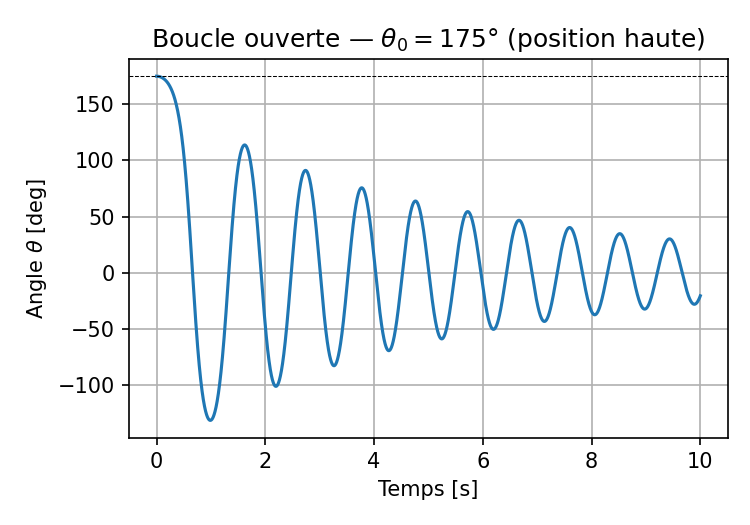
\includegraphics[width=\linewidth]{figures/openloop_175deg.png}
  \end{figure}
\end{column}

\end{columns}

\end{frame}

%%%%%%%%%%%%%%%%%%%%%%%%%%%%%%%%%%%%%%%%%%%%%%%%

\begin{frame}
\frametitle{Étude de la dynamique}
\framesubtitle{Comparaison modèle / expérience}

\begin{center}
\begin{tikzpicture}[>=Stealth,
    box/.style={draw, rounded corners=4pt, fill=blue!8, text width=2.8cm,
                align=center, minimum height=1.2cm, font=\small},
    arr/.style={->, thick, blue!60!black}
  ]

  \node[box] (meas) {Mesure de la\\réponse\\expérimentale};
  \node[box, right=1.2cm of meas] (opt)  {Optimisation\\des paramètres\\du modèle};
  \node[box, right=1.2cm of opt]  (res)  {Paramètres\\identifiés\\$m,\ l,\ c$};

  \draw[arr] (meas) -- (opt);
  \draw[arr] (opt)  -- (res);

\end{tikzpicture}
\end{center}

\vspace{0.2cm}

\begin{figure}
    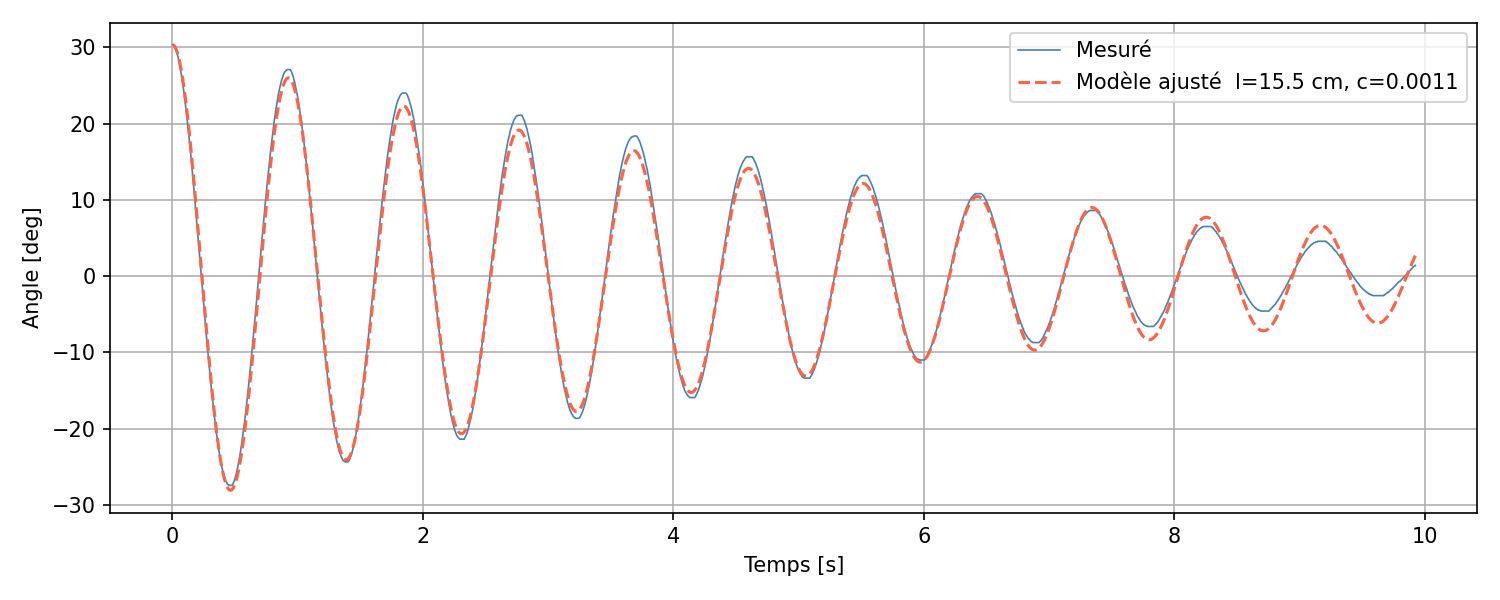
\includegraphics[width=\linewidth]{figures/free_response_fit.png}
\end{figure}

\end{frame}
